\chapter{Implementierung}
\label{chap:Implementierung}

\section{Architektur}

Nachfolgend wird der derzeitige Stand der Architektur der Anwendung beschrieben. Da dies lediglich der erste Teil einer gr\"oßeren Arbeit ist, 
k\"onnen infolge des zweiten Teils der Arbeit Ver\"anderungen an der Architektur auftreten. 

Wie in Abschnitt~\ref{subsec:OSGi} bereits angesprochen, wird die Anwendung unter Verwendung von OSGi~\footnotemark[1] umgesetzt. 
Als Implementierung des OSGi-Standard wurde im Rahmen dieser Arbeit das Framework \gls{Equinox}~\footnotemark[2] gew\"ahlt. 
Die Eclipse IDE und die von jnect verwendeten Frameworks basieren ebenfalls auf dieser Plattform, sie ist daher optimal geeignet. 
Durch Implementierung der Gesten, Sprachbefehle und Aktionen durch OSGi-Bundles~\footnotemark[3] ist es m\"oglich zur Laufzeit 
der Anwendung neue Gesten nachzuladen oder Aktionen neu zu definieren. Geschaffen wird diese lose Kopplung der Komponenten durch 
die Nutzung der Service-Funktionalit\"at der OSGi-Plattform.

In Abbildung~\ref{fig:osgiArchitecture} ist die aktuelle Architektur der Anwendung zu sehen. In Abschnitt~\ref{sec:osgiBundles} werden 
die dargestellten Komponenten n\"aher beschrieben. Die Komponenten stellen ihre Funktionalit\"at in Form von Services~\footnotemark[3] bereit. 
Ein Service wird mittels eines Interface am Framework registriert. Somit k\"onnen andere Bundles einen Service nutzen, ohne dessen konkrete 
Implementierung kennen zu m\"ussen.

\footnotetext[1]{Osgi Alliance (2013) \href{http://www.osgi.org/Technology/HomePage}{\textit{OSGi Alliance}} osgi.org, Abgerufen Januar 07, 2013}
\footnotetext[2]{The Eclipse Foundation (2013) \href{http://www.eclipse.org/equinox/}{\textit{Eclipse Equinox}} eclipse.org, Abgerufen Januar 07, 2013}
\footnotetext[3]{Osgi Alliance (2013) \href{hhttp://www.osgi.org/Technology/WhatIsOSGi}{\textit{OSGi Technology}} osgi.org, Abgerufen Januar 07, 2013}

\begin{figure}[htb]
\centering
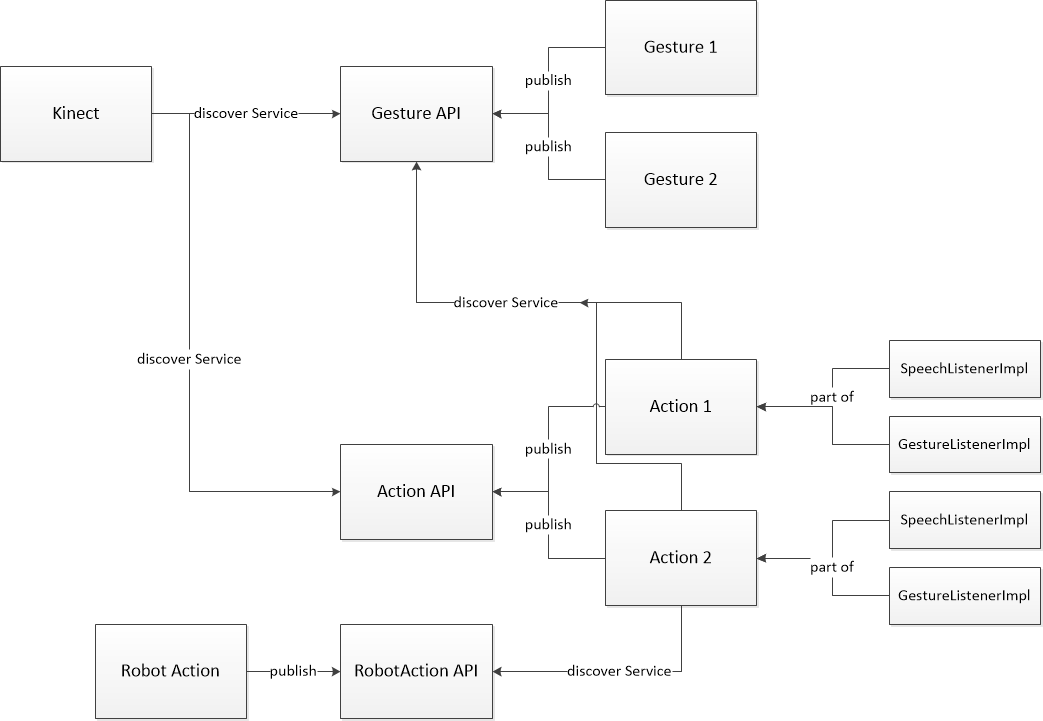
\includegraphics[width=1\textwidth]{img/09kapitel/osgi-architecture.png}
\caption[Anwendungsarchitektur]{Architektur der Anwendung}
\label{fig:osgiArchitecture}
\end{figure}

\section{Bundles}
\label{sec:osgiBundles}

Bundles stellen ihre Funktionalit\"at mittels Services zur Verf\"ugung. Dies geschieht mittels eines Interface. 
Das Interface wird in einem eigenen Bundle definiert. Hierdurch entsteht eine statische Abh\"angigkeit 
zwischen einem API-Bundle und seinen implementierenden Bundles. Dieser wird geschaffen mittels der Deklaration von importierten 
und exportierten Bundles im Manifest des Bundles (Abbildung~\ref{listing:manifestGestureAPI}). Die OSGi-Runtime liest beim Start 
eines Bundles das Manifest ein und l\"ost die Abh\"angigkeiten auf. Ist dies nicht m\"oglich, kann ein Bundle nicht gestartet werden. 
Ebenso k\"onnen laufende Bundles wieder beendet werden. Hierf\"ur existiert das Konzept des Bundle-Lifecycle~\footnotemark[3].

\newpage
\par\smallskip
\lstset{language=Java}
\begin{lstlisting}[caption={Manifest der Gesture API}, label={listing:manifestGestureAPI}]
Manifest-Version: 1.0
Bundle-ManifestVersion: 2
Bundle-Name: Rocovomo Gesture API
Bundle-SymbolicName: de.rocovomo.jnect.gesture
Bundle-Version: 0.0.1.qualifier
Bundle-RequiredExecutionEnvironment: JavaSE-1.7
Import-Package: org.eclipse.emf.common,
 org.eclipse.emf.ecore,
 org.jnect.gesture
Export-Package: de.rocovomo.jnect.gesture.api,
 de.rocovomo.jnect.gesture.provider.api
\end{lstlisting}
\par\smallskip

\subsection{Kinect}

Das Kinect-Bundle hat Abh\"angigkeiten zu den jnect-Bundles. In dieser Komponente wird die Anbindung zur Kinect implementiert. Dieses Bundle 
sucht nach Services, welche durch die Gesture- und Action-Bundles zur Verf\"ugung gestellt werden. Es registriert Gesten, sowie die 
Gesten-Listener und Sprach-Listener der Action-Bundles an der Kinect. Durch die Listener erhalten die Action-Bundles die Information 
ob sie ausgel\"ost wurden. Das Bundle stellt die effiziente Verwaltung von Gesten und Listenern sicher, sowie die Verwaltung der 
angeschlossenen Kinect. Ohne das Kinect for Windows \acrshort{SDK} kann dieses Bundle nicht gestartet werden.

\subsection{Gesture}

In den Gesture-Bundles werden Gesten implementiert. Finden Ver\"anderungen im Modell statt, so wird dies den Gesture-Bundles mitgeteilt und 
diese analysieren mittels HMMs ob sie ausgel\"ost wurden. Gesten stellen sich als Service zur Verf\"ugung. Sie werden vom Kinect-Bundle zur 
Erkennung verwendet. Auch die Action-Bundles m\"ussen ihre entsprechenden Gesten kennen. Gesten werden als unabh\"angige Bundles von Aktionen 
realisiert. Hierdurch wird eine Codeduplikation bei Aktionen die gleiche Gesten verwenden vermieden.

Die Implementierung einer Geste muss von der jnect-Klasse \textit{Gesture}~(Listing \ref{listing:Gesture}) erben. In der Methode 
\textit{isGestureDetected(\ldots)} wir das HMM zur Erkennung der Geste implementiert. Ist die Gesten am Gesten-Proxy der Kinect 
angemeldet, so wird der \textit{GestureListener}, welcher diese Geste nutzt aufgerufen.

\par\smallskip
\lstset{language=Java}
\begin{lstlisting}[caption={Klasse Gesture}, label={listing:Gesture}]
public abstract class Gesture extends EContentAdapter {

	private GestureProxyCallback gestureProxy;

	/**
	 * DO NOT CALL THIS METHOD, IT WILL BE CALLED BY THE GESTUREPROXY
	 * 
	 * @param gestureProxy
	 *            the proxy to notify when a gesture is detected
	 */
	public void setGestureProxy(GestureProxyCallback gestureProxy) {
		this.gestureProxy = gestureProxy;
	}

	@Override
	public void notifyChanged(Notification notification) {
		if (gestureProxy != null && isGestureDetected(notification)) {
			this.gestureProxy.notifyGestureDetected(this.getClass());
		}
	}

	/**
	 * checks whether the searched gesture is detected
	 * 
	 * @param notification
	 *            the notification containing the model changes
	 * @return true if the gesture was detected
	 */
	protected abstract boolean isGestureDetected(Notification notification);
}
\end{lstlisting}
\par\smallskip

\subsection{Action}
\label{subsec:osgiaction}

Die Action-Bundles bilden einen Befehl ab. Dieser Befehl kann entweder eine Geste, ein Sprachbefehl oder eine Kombination aus beidem sein. 
Je nachdem verf\"ugt die Action \"uber einen \textit{Speech}- oder einen \textit{GestureListener}. Eine Kombination aus beidem ist hier 
auch m\"oglich. Die Integration dieser beiden Eingabeoptionen wird von Buxton~\cite{bib:buxton}~\footnotemark[4] in Form von Frames besprochen. 
Eine Aktion ist abh\"angig von einer Geste die von einem Gesture-Bundle bereitgestellt wird.

Wird eine Geste erkannt wird die Methode \textit{notifyGestureDectected(\ldots)} der entsprechenden Implementierung der abstrakten Klasse
\textit{GestureListener} (Listing~\ref{listing:GestureListener}) aufgerufen. Von hier kann dann die entsprechende Roboter-Aktion aufgerufen werden.

Das Vorgehen ist beim \textit{SpeechListener}~(\ref{listing:SpeechListener}) prinzipiell \"ahnlich. Wird ein Sprach-String der Implementierung
des \textit{SpeechListener} erkannt, so wird die entsprechende Methode, \textit{notifySpeech(\ldots)} aufgerufen. Im Gegensatz zur Geste ist die
Sprache weniger komplex und wird nur mittels Strings definiert. Diese erh\"alt der \textit{KinectManager} mittels \textit{getWords(\ldots)}.

Bislang stellt sich das Action-Bundle selbst als Service zur Verf\"ugung. Das Kinect-Bundle erh\"alt so Zugriff auf die \textit{Speech-} und 
\textit{GestureListener}.

\footnotetext[4]{Kapitel 14 Multimodal Integration}

\par\smallskip
\lstset{language=Java}
\begin{lstlisting}[caption={Klasse GestureListener}, label={listing:GestureListener}]
public abstract class GestureListener {

	/**
	 * callback method, that gets called when a {@link Gesture} is detected
	 * 
	 * @param gesture
	 *            - the class of the {@link Gesture} that was detected
	 */
	public abstract void notifyGestureDetected(Class<? extends Gesture> gesture);

	/**
	 * {@link Set} of {@link Gesture}s this {@link GestureListener} listens to
	 * 
	 * @return {@link Set} of {@link Gesture}s to be notified about, can be
	 *         empty but not null
	 */
	public Set<Gesture> getGestures() {
		return Collections.emptySet();
	}

	/**
	 * Whether the {@link GestureListener} listens only to special
	 * {@link Gesture}s.
	 * 
	 * @return true if only the {@link Gesture}s provided in
	 *         {@link #getGestures()} should be provided to the listener, false
	 *         otherwise
	 */
	public boolean isFiltered() {
		return false;
	}
\end{lstlisting}
\par\smallskip

\par\smallskip
\lstset{language=Java}
\begin{lstlisting}[caption={Klasse SpeechListener}, label={listing:SpeechListener}]
public abstract class SpeechListener {
	/**
	 * callback when a relevant speech is recognized
	 * 
	 * @param speech
	 *            - the speech recognized
	 */
	public abstract void notifySpeech(String speech);

	/**
	 * a set of words that this {@link SpeechListener} wants to be recognized
	 * and notified about
	 * 
	 * @return a {@link Set} of {@link String}s building the relevant words
	 */
	public abstract Set<String> getWords();

	/**
	 * if a {@link SpeechListener} is filtered than it will be only notified
	 * about recognized words that are contained in the {@link Set} provided by
	 * {@link #getWords()}
	 * 
	 * @return true if should be filtered, false otherwise
	 */
	public boolean isFiltered() {
		return true;
	}
}
\end{lstlisting}
\par\smallskip

\subsection{Robot Action}
\label{subsec:Roboterschnittstelle}

Bundles, welche die Robot Action \acrshort{API} implementieren, stellen sich ebenfalls als Services zur Verf\"ugung. Action-Bundles stellen auf dieser 
Basis eine Verbindung zwischen Geste/Sprachbefehl und Roboter-Aktion her. Grunds\"atzlich k\"onnte man dies auch umgekehrt konstruieren, dass
sich die Roboter-Aktion ein passendes Action-Bundle sucht. Da Roboter-Interaktion Teil des zweiten Teils der Arbeit ist, ist dieses Bundle 
bisher noch ohne jede Funktionalit\"at.

\section{User Interface}

Als User-Interface ist eine Anwendung auf Basis der \gls{RCP} von Eclipse vorgesehen. Zur Visualisierung der 
der Eingaben des Nutzers war eine dreidimensionale Umgebung mit Hilfe der \gls{LWJGL} vorgesehen. 
Optisch orientiert sich eine Anwendung auf dieser Plattform am Aussehen der Eclipse IDE, zu sehen in Abbildung~\ref{fig:eclipse}. 
Bislang kann das Skeleton-Modell in einem GEF-Editor dargestellt werden, dies wurde in Abbildung~\ref{fig:gef} bereits gezeigt. Erkannte Gesten und Sprachbefehle werden bislang auf einer Logging-Konsole
ausgegeben.

\begin{figure}[htb]
\centering
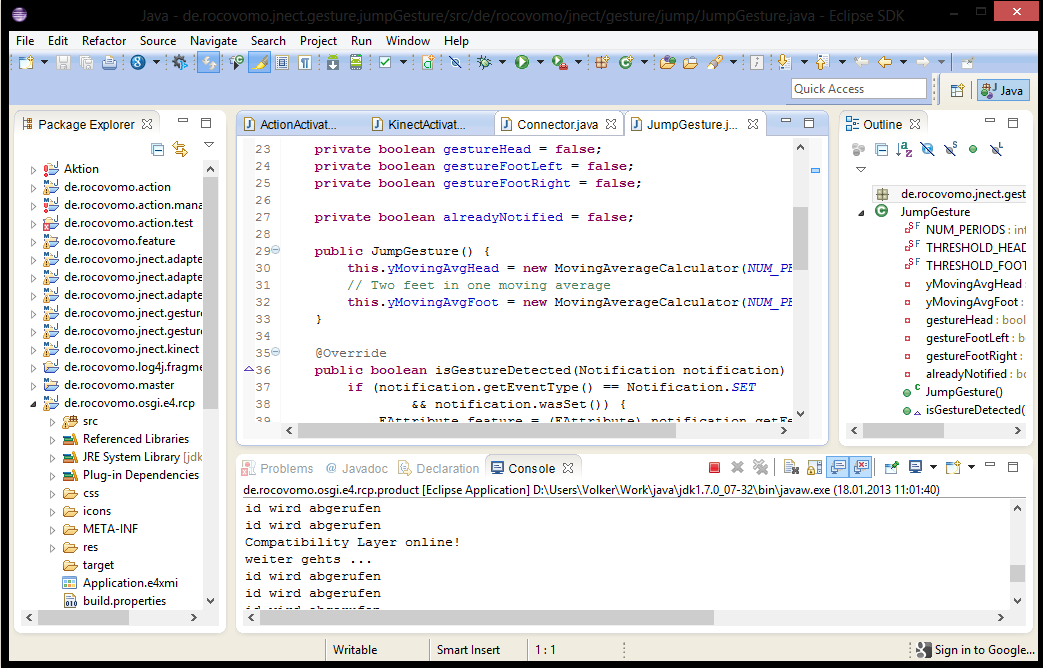
\includegraphics[width=1\textwidth]{img/09kapitel/rcp.png}
\caption[Eclipse IDE]{Eclipse IDE}
\label{fig:eclipse}b
\end{figure}

